\documentclass[9pt,twocolumn,twoside]{pnas-new}
% Use the lineno option to display guide line numbers if required.
% Note that the use of elements such as single-column equations
% may affect the guide line number alignment. 

\templatetype{pnasresearcharticle} % Choose template 
% {pnasresearcharticle} = Template for a two-column research article
% {pnasmathematics} = Template for a one-column mathematics article
% {pnasinvited} = Template for a PNAS invited submission

\title{Collision detection for multiple serial manipulators}

% Use letters for affiliations, numbers to show equal authorship (if applicable) and to indicate the corresponding author
\author[a,b,1]{Brian Cohn}
\affil[a]{University of Southern California, Department of Computer Science}
\affil[b]{brian.cohn@usc.edu}

% Please give the surname of the lead author for the running footer
\leadauthor{Cohn} 

% Please add here a significance statement to explain the relevance of your work
\significancestatement{Manipulators are used primarily in the manufacturing industry, but will become more typical as cost is reduced and algorithms become more reliable. These robots can be mounted to the ground for heavy industrial work (such as manipulation of automobile frames) or connected to small robots to allow for precise dexterous manipulation of objects. As more robots are developed, it will become increasingly important to predict and avoid collisions between manipulators---this will help keep maintenance costs down, improve multi-robot collaboration tasks, and improve safety metrics.}

% Please include corresponding author, author contribution and author declaration information
\authordeclaration{The author declares no conflicts of interest.}
\correspondingauthor{\textsuperscript{2}To whom correspondence should be addressed. E-mail: brian.cohn@usc.edu}

% Keywords are not mandatory, but authors are strongly encouraged to provide them. If provided, please include two to five keywords, separated by the pipe symbol, e.g:
\keywords{manipulation $|$ mobile coordination $|$ robotics $|$ collision detection} 

\begin{abstract}
Although we know a lot about collision detection in small systems of up to three manipulators, the field has a gap: we do not have collision detection algorithms for five or more serial manipulators. A model that can quickly validate a prospective task across a group of robots would significantly advance the field, but it has not received much attention. This paper introduces an efficient algorithm for preventing multi-manipulator collisions, that is readily parallelizable at multiple levels of abstraction. Five simulated manipulators, with three links, were each asked to reach an endpoint target using elementary inverse kinematics. For each position set, the collision detection algorithm is capable of identifying whether any pairs of arms would intersect, without the complexity of considering the overall thickness and shape of each segment of the arm. This allows for further collision detection with other available algorithms, but only for the ones that get past the line intersection test. While this method does not increase the speed of traditional collision detection algorithms, it reduces the number of calls to existing approaches by only having them evaluate candidate positions that have been pre-vetted.
\end{abstract}

\dates{This manuscript was compiled on \today}
\doi{\url{www.my.usc.edu/doi/10.1073/usc.XXXXXXXXXX}}

\begin{document}

% Optional adjustment to line up main text (after abstract) of first page with line numbers, when using both lineno and twocolumn options.
% You should only change this length when you've finalised the article contents.
\verticaladjustment{-2pt}

\maketitle
\thispagestyle{firststyle}
\ifthenelse{\boolean{shortarticle}}{\ifthenelse{\boolean{singlecolumn}}{\abscontentformatted}{\abscontent}}{}

% If your first paragraph (i.e. with the \dropcap) contains a list environment (quote, quotation, theorem, definition, enumerate, itemize...), the line after the list may have some extra indentation. If this is the case, add \parshape=0 to the end of the list environment.
\dropcap{S}erial manipulators are highly versatile and deft robots. Understanding the way they interact with a \textit{task} is just as important as comprehending \textit{interactions} among manipulators. Increasing the speed or accuracy of robotic control has opened up new opportunities for more complex behavior and interaction. Many of the path planning algorithms in the literature focus on collaborative tasks, such as moving one object. Collision detection for multi-manipulator link systems is often laborious, as each manipulator consists of multiple connected obstacles for its fellow manipulators.
\\
The aim of this paper is to close the gap on collision detection in multi-manipulator robotic systems. As such, the primary research questions of this paper that are sought are:
\begin{enumerate}
  \item Is a line segment algorithm computationally sufficient in predicting collisions?\\
  \item What is the relationship between manipulator \textit{anchor position} and the probability of a prospective position having a collision? \\
  \item Does the speed of this approach make it conducive to computationally-tractable applications?\\
\end{enumerate}

\subsection*{Approach and Methods}



\subsubsection*{Sampling points for feasible positions}
Each task is defined as a set of $n$ points, each with an $x$ and $y$ floating point value, to represent the list of targets for the five manipulators. Each manipulator has the same shape for its workspace, but rather than computing the complex workspace, I decided to sample feasible tasks from an annulus that was fixated at the center of each manipulator. This reduces the number of solutions that that have to be verified, while still providing an adequate sampling of the workspace.

\begin{figure}%[tbhp]
\centering
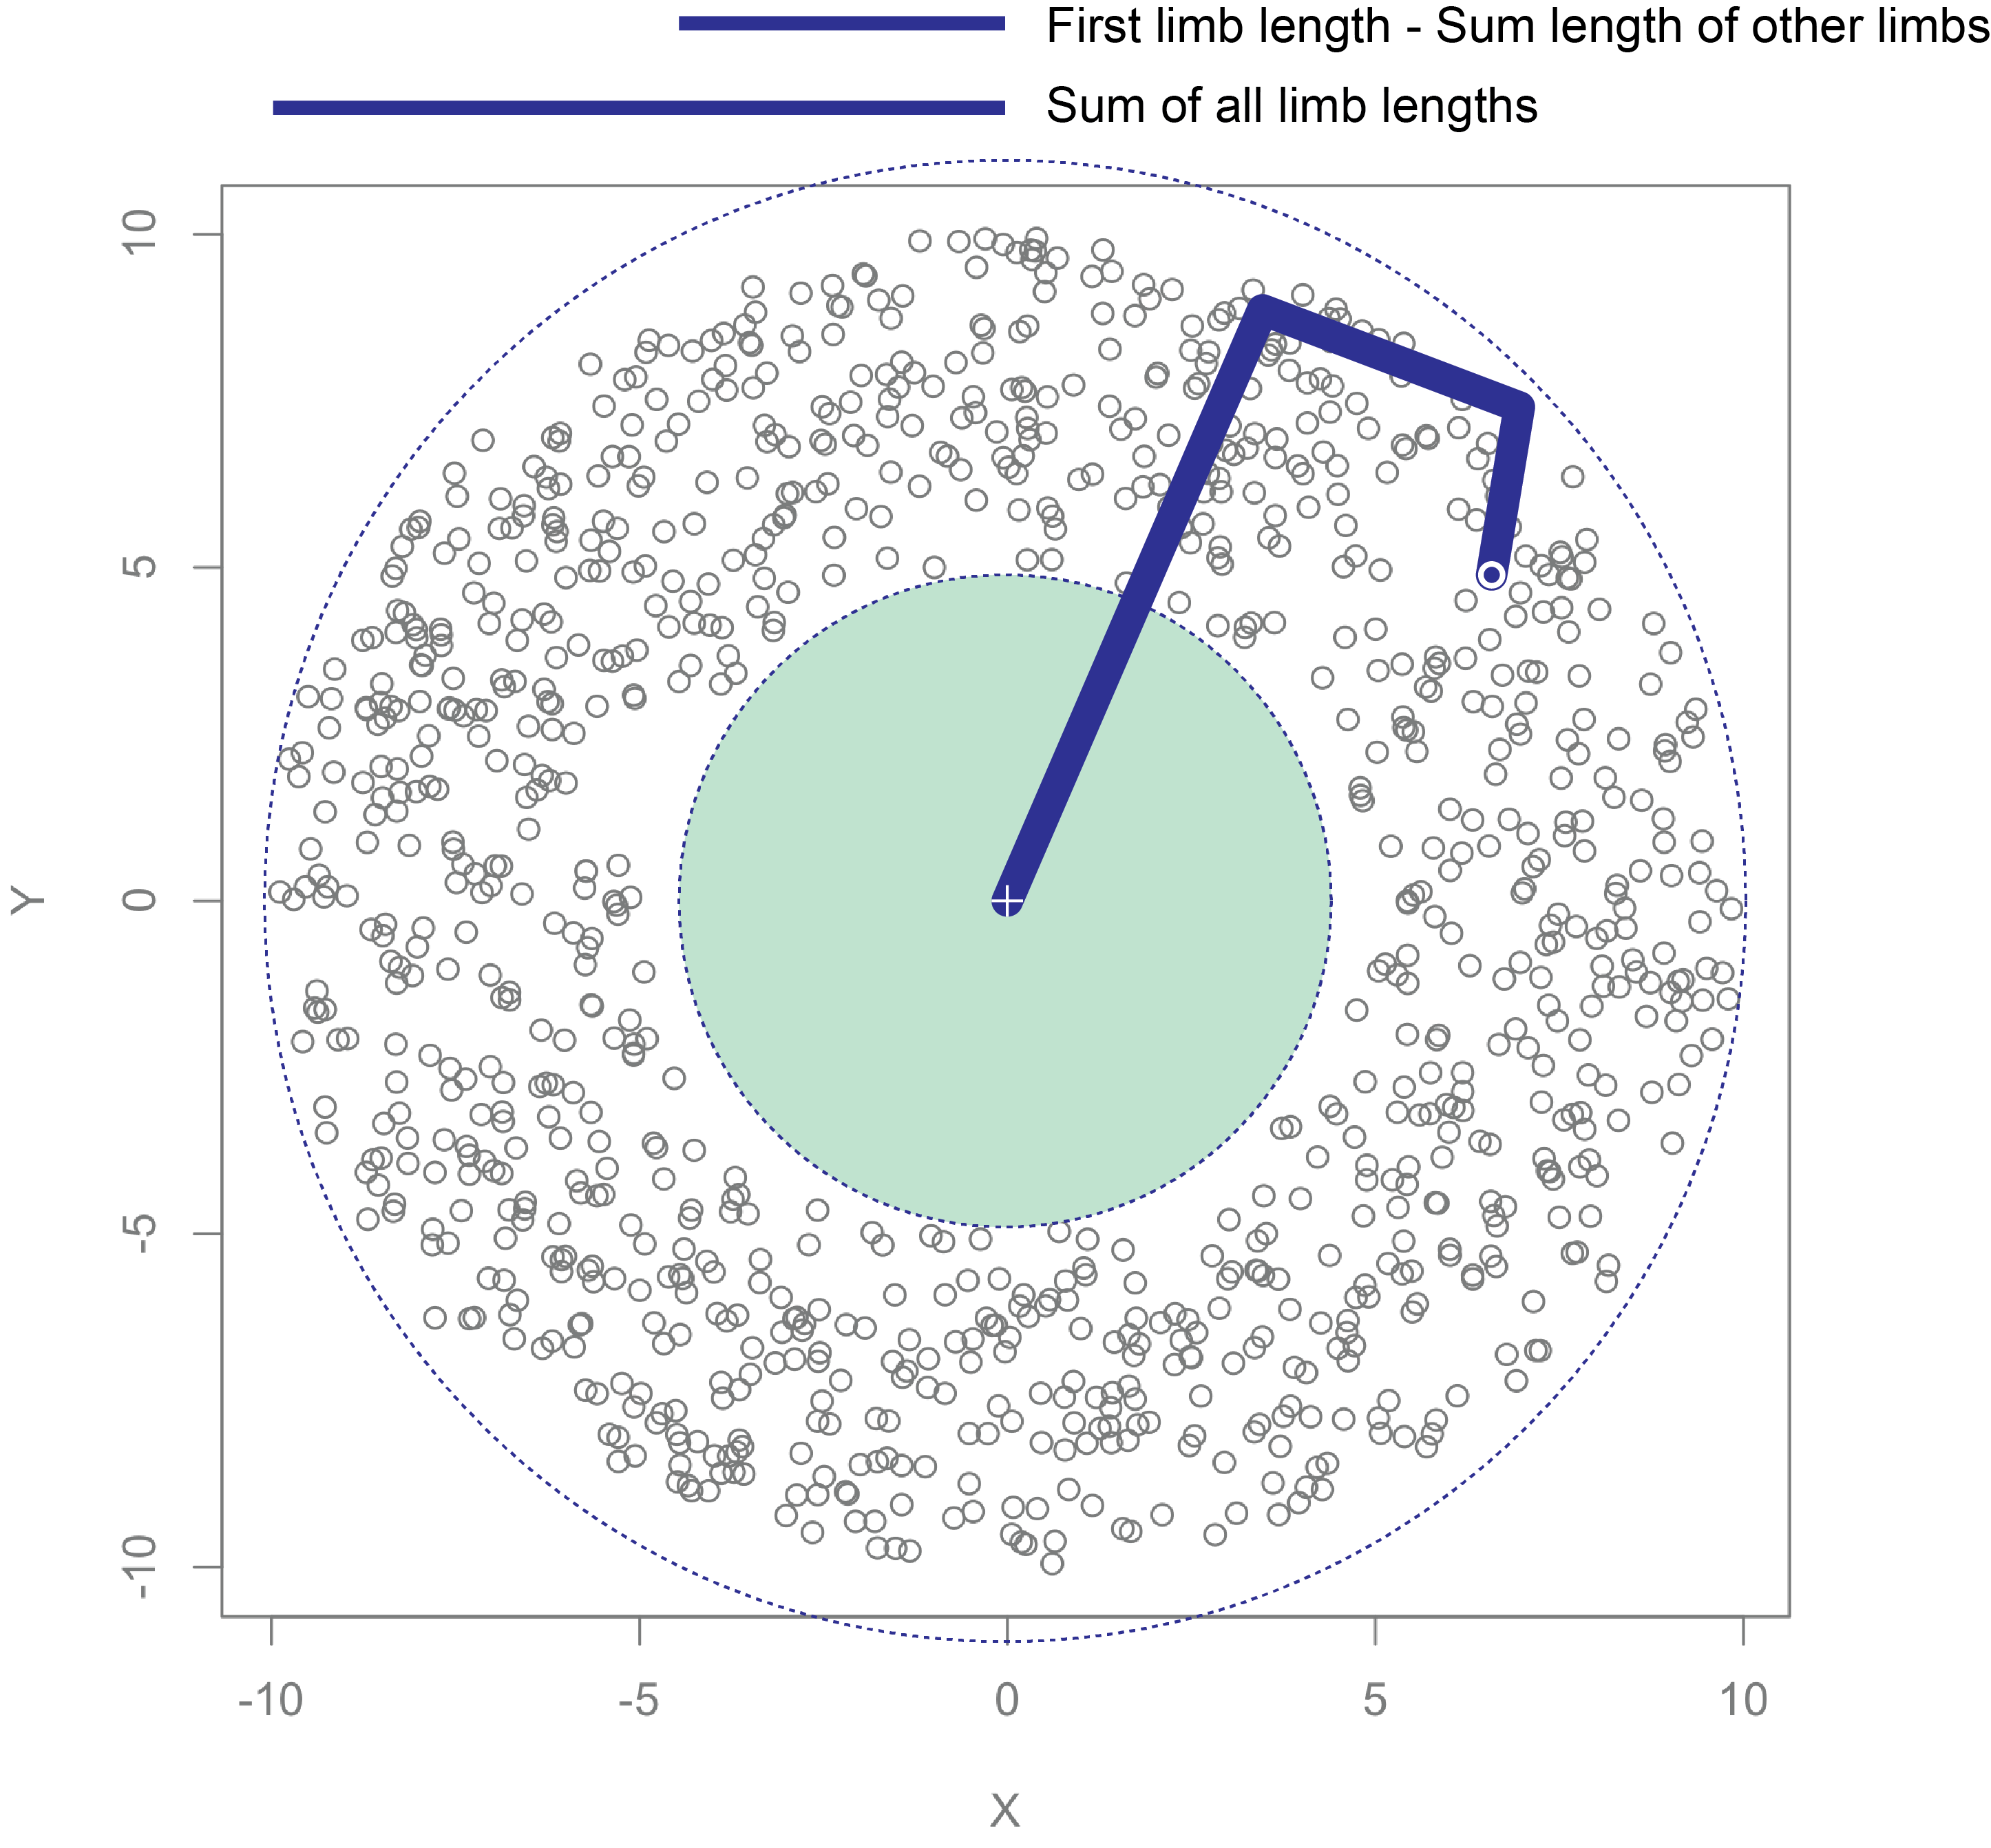
\includegraphics[width=.8\linewidth]{manipulator_subsample_points}
\caption{Example points given to one of the manipulators across 1000 trials, where the manipulator's first link length was 5cm. Each manipulator is presented one prospective position per trial---these points are sampled u.a.r from a square, and samples generated outside the desired ring were excluded. See the \textit{uar\_sample\_from\_circle} function and it's helper function entitled \textit{point\_is\_in\_ring}. Points were excluded from the inner ring because those are regions which are difficult for the manipulator to adequately target.}
\label{fig:points}
\end{figure}

The manipulators are not well suited to reach the inside of the circle, so removing the inner radius was a quick way to significantly reduce the computation time---there is no need to run the inverse kinematics on positions that are provably impossible (Fig. \ref{fig:points}). \\Similarly, the outer radius is designed to remove all points that are impossible because they extend too far beyond the cumulative length of all segments. In the figure I show an example where the outer radius is smaller than the cumulative length. All simulations were performed at an outer radius $:=$ the manipulator's feasible working area, and the inner radius $:=$ the first link minus the other two link lengths to prevent highly acute joint angles that are unreasonable in application.\\
\subsubsection*{Inverse Kinematics}
I began with an inverse kinematics model developed by the StudyWolf blog. This was set up to generate one 3-link Arm. I added a parameter to define the $x,y$ displacement of a given manipulator's anchorpoint by changing the homogenous transformation matrix, and highly modularized the code so I could extend it in the following ways:

\begin{itemize}
  \item Extended the information held within the Arm class to include endpoint locations, limb segments, and endpoint errors
  \item Designed a plotting interface to quickly view multiple arms in the same environment
  \item Built a set of list-comprehensions that can be readily parallelized due to its functional nature
\end{itemize}

The third point is particularly significant, because it shows how quickly the algorithm can be put on-board a manipulator's CPU to be a local algorithm. That way, a manipulator would only be responsible for computing the feasible collisions with it's nearest neighbors. This level of modularization is especially important when designing systems with heterogeneous types of robots, as each robot has it's own requirements and geometries.

\subsubsection*{Collision detection}
Each manipulator has 3 links, and one of the links has an end that is anchored to a single point. That leaves two joints connected to three line segments representing the links. With five manipulators, and a total of 15 segments, there are $n=_{15}C_{k=3}$ total combinations to evaluate. This ends up being relatively fast on modern CPU architectures.\\ 
By leveraging Cramer's rule, we are able to identify whether two line segments intersect. This implementation of Cramer's rule is derived from \cite{stackoverflowanswer}.
We first begin with the linear system of equations that represent two line segments.
%% Do not use widetext if paper is in single column.
% \begin{widetext}
\begin{align*}
A_1 * x + B_1 * y = C_1\\
A_2 * x + B_2 * y = C_2
\end{align*}
% \end{widetext}

And next, compute $x$ and $y$ independently, to identify where the intersection lies (if it exists).
\begin{align*}
(x,y) = \left(\frac{D_x}{D}, \frac{D_y}{D}\right)
\end{align*}
Where $D$ is the determinant of the system of linear equations, and $D_i$ represents the coefficient determinant where the values in column $i$ are overwritten with the values in the answer-column \cite{strang2011introduction}. 

Finally, I identify whether the point is on one of the line segments, or if it is on the infinite line extrapolated beyond the endpoints. If between the two points, the two links are noted as a collision.
\\
\subsubsection*{Implementation}
Functions were implemented within two files: \textit{Arm.py} and \textit{main.py}. \textit{Arm.py} held the Arm class, where I instantiated the angles for each of the limb segments, defined the lengths of the limbs, and defined the location of the anchorpoint. I added many methods within this class, such as \textit{snap\_arm\_to\_new\_XY\_target}, which applies a random point from the annulus to the arm, and uses the inverse kinematics transformation 
See the detailed function descriptions in the source code repository at \href{https://github.com/bcohn12/robo-movement-feasibility}{GitHub Repository}.
All algorithms were developed in Python 3.3.5, highly leveraging the SciPy distribution for numerical simulation, and focusing on a functional approach so the implementation could be parallelized at the controller or the local level.

\subsection*{Results and evaluation}
\begin{figure}%[tbhp]
\centering
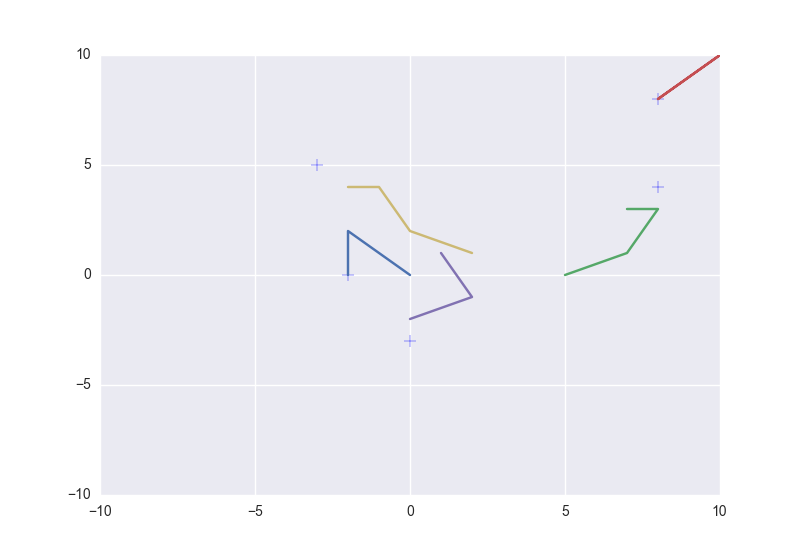
\includegraphics[width=1.0\linewidth]{file1480904553866_949}
\caption{An example of a non-colliding set of manipulators that resulted from the stochastic simulation. The anchorpoints of these manipulators were placed at random about the XY plane. Limb lengths and capabilities are homogenous across the five manipulators. Endpoint positions and limb lengths are described in integer values, and can be readily increased to improve the system's precision. Each manipulator is a different color, and the plus marks the target endpoint positions for each manipulator.}
\label{fig:trials}
\end{figure}


\begin{figure}%[tbhp]
\centering
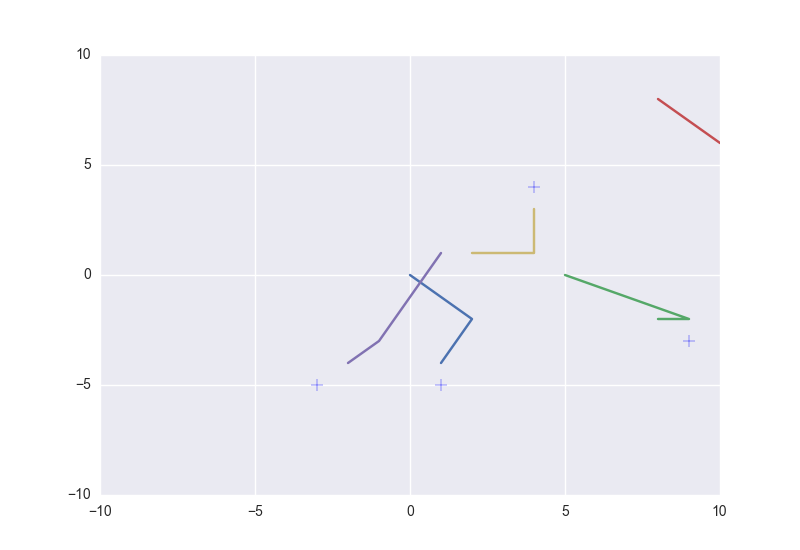
\includegraphics[width=1.0\linewidth]{file1480904545447_182}
\caption{An example of manipulator collision between the blue and purple-colored manipulators at the center of the work space.}
\label{fig:nonintersection}
\end{figure}


\begin{SCfigure*}[\sidecaptionrelwidth][t]
\centering
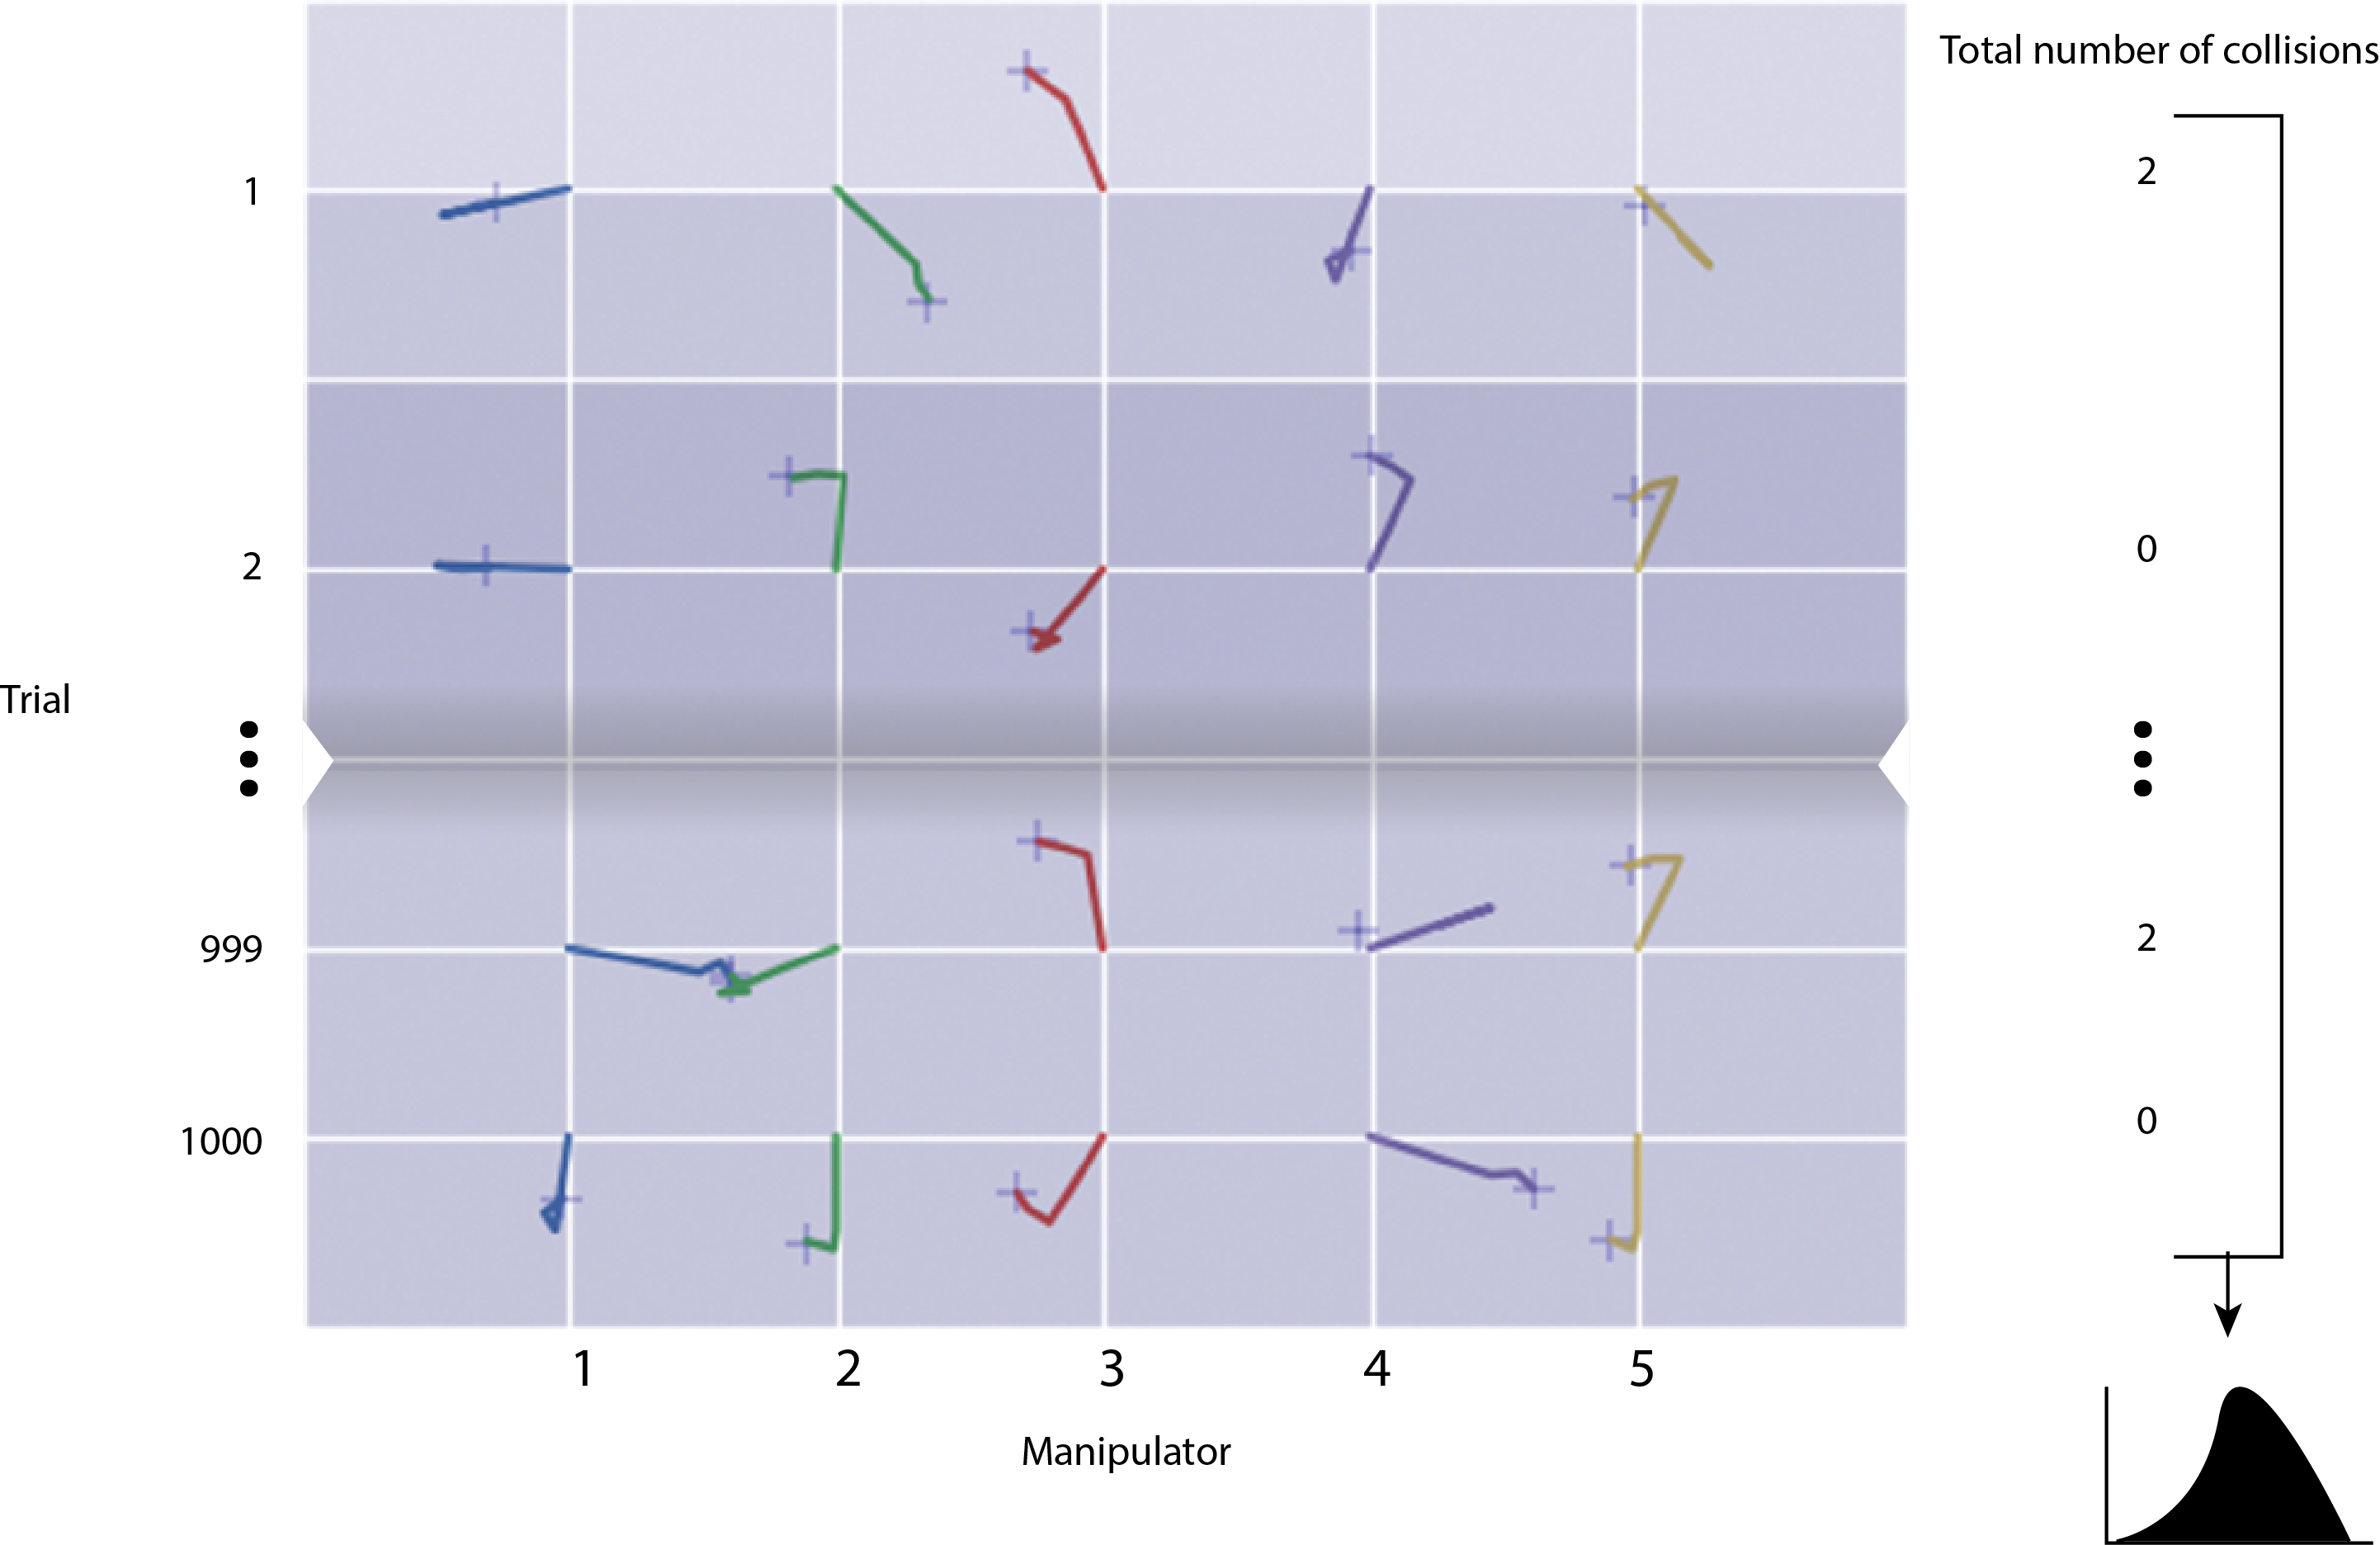
\includegraphics[width=11.4cm]{trial_explanation}
\caption{One thousand position vectors are selected for each trial. A position vector represents the desired $(x,y)$ coordinate that each of the manipulators is targeting. For each trial, we compute the total number of collisions. The vector of collision totals are concatenated to produce the histograms seen in later figures.}\label{fig:intersection}
\end{SCfigure*}

The linear algebra approach to line segment collision detection was successful, and the collisions were validated visually and numerically for 3 edge cases (Fig. \ref{fig:intersection}). A smaller portion of the generated positions were valid; one such example is shown in Fig. \ref{fig:nonintersection}.
\begin{SCfigure*}[\sidecaptionrelwidth]
\centering
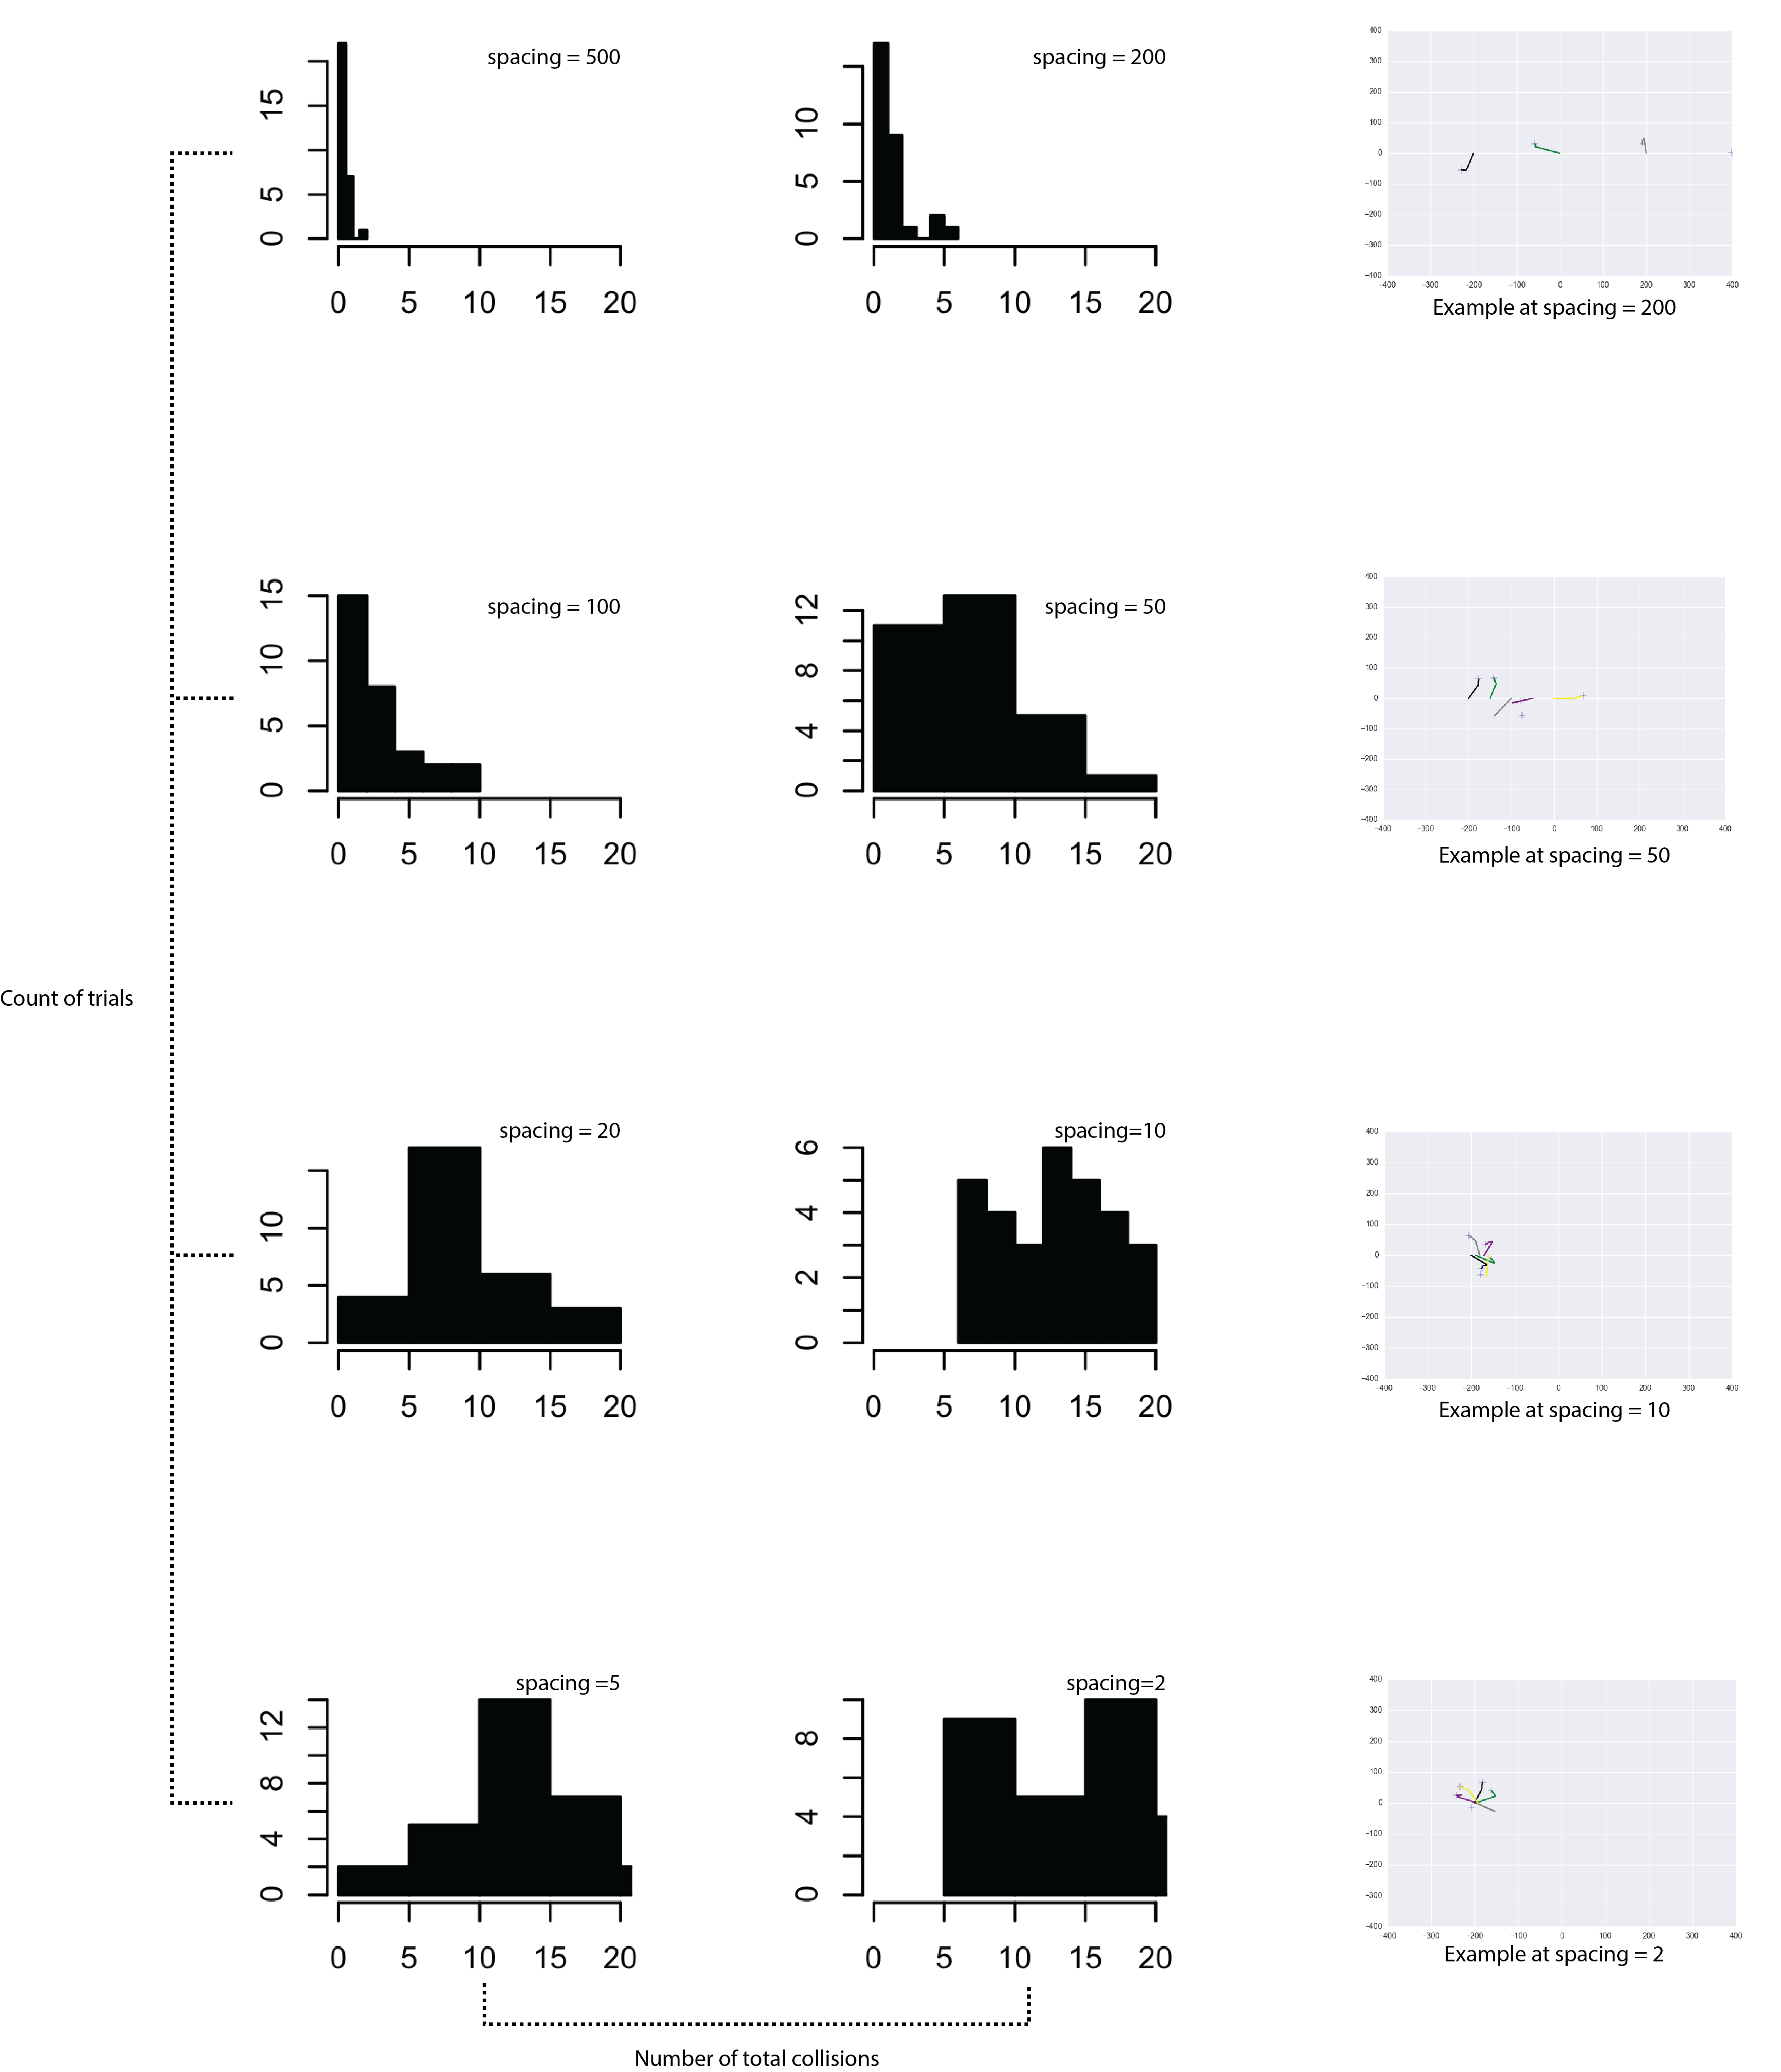
\includegraphics[width=11.4cm]{collision_histograms}
\caption{As spacing gets closer, the likelihood of collision increases. These histograms illustrate how organizing manipulators in a 2D space affecst the likelihood that a stochastically-chosen posture will be viable.}\label{fig:histograms}
\end{SCfigure*}
Using a progression of decreasing anchor distances between manipulators, from 200 to 0 cm, I collected the total number of collisions for each value of anchor spacing. I computed a histogram at each vector, to illustrate the change in the collision likelihood as manipulators get closer (Fig. \ref{fig:histograms}).

No statistical tests were run to compare the differences in means across groups, though the data appear conducive to post-hoc analyses.

\subsection*{Strengths and Weaknesses}

This application is highly endpoint-space focused, and holds up in comparison to other biologically-inspired approaches \cite{teja2016learning}, and has a rigorous mathematical basis. While this algorithm does not serve as a comprehensive planner, it can reduce a significant amount of time spent searching, because it can remove entire sections of the feasible path set. In a random search algorithm that's looking for a viable multi-robot path, it can use this paper's approach as a way to ignore high-collision situations. As this method only looks at line intersections, it does not represent any mass or volume of the serial links. \\If this verification were applied to a set of prospective positions, it would return an ambitious set of possible positions---from there, one would have to compute more complicated collision detection approaches on the remaining solutions. The histogram distributions show a surprisingly distributed effect of decreasing inter-manipulator spacing, and this may have implications on the design of future collaborative multi-manipulator systems.
\\
Another weakness of this approach is that it does not distinguish between an arm-arm collision and a collision within a single manipulator arm. It's important for an individual controller to understand it's kinematic and static capabilities from the standpoint of joint space. While this feature is typically built into many on-line contol algorithms, it is not covered in my approach.
\\
With regards to accuracy, if the inverse kinematics is changed, then this model will continue to work. For any controller that predicts the orientation it will reside at, the line segment analysis will be valid. However, the inverse kinematic algorithm I used is highly temperamental---many times it does not find a solution to the problem because the matrix becomes singular; this is visible through visualizations where some of the manipulators are pointed in the exact opposite direction of their target, or are completely outstretched in an erroneous direction. This error could be mitigated through the application of an inverse kinematics approach that handles singularity more deftly.

\begin{table}%[tbhp]

\caption{Benchmark performance of the line segment collision detection algorithm on five manipulators indicates near-linear scaling.} \label{tab:a}
\begin{tabular}{lrrr}
\centering
Number of positions checked & Elapsed Time (seconds) \\
\midrule
1 & 00.055883 \\
10 & 00.583959 \\
100 & 05.512406 \\
1000 & 56.615337 \\
\bottomrule
\end{tabular}
\end{table}

This performance table illustrates how many positions can be evaluated on one thread on a modern computer. This indicates a nearly-linear Big O(N) algorithmic implementation, where N is the number of prospective values to evaluate. This approach can be divided by however many cores the tasks are distributed to.




\subsection*{Related Work}
Considering that each manipulator has it's own positioning, variance, noise, and it's own task to perform, selecting a good path is nontrivial. Safety concerns have to be put into the equation when manipulators interact with human counterparts \cite{Jung2014}. Decreasing the time to compute collision verification will advance the capability for robots to collaborate without crashing into obstacles, people, and one another---extending new applications for attaching manipulators to mobile robots and integrating heterogenous manipulators.
\\
The state of the art in collision detection algorithms range from the "most generic collision detection algorithms" that can be applied "to only polygonal meshes or objects of convex primitives"\cite{Li:2012bn}, all the way to a spring-damper field atop the equation of motion for the endpoint\cite{Stadlbauer:2008ky}. 
\\
\begin{table}%[tbhp]

\caption{Notes on eight papers that surround this paper's topic} \label{tab:a}
\begin{tabular}{lrrr}
\centering
Reference Number & Description \\
\midrule
1. \cite{sunada1994coordinated} & Control of a three-armed robot \\
2. \cite{korayem2016sdre} & Wheeled mobile cooperative manipulator \\
3. \cite{sun2016safe} & Random tree search algorithm for a tentacle-like robot \\
4. \cite{hsu1993coordinated} & One manipulator on a screw, another on a bolt \\
5. \cite{khatib1996vehicle} & Multi-arm robots with fixed bases \\
6. \cite{baizid2016behavioral} & 6DOF manipulator attached to an airplane \\
7. \cite{hsu1993adaptive} & Theoretical approach with adaptive trajectory planning \\
8. \cite{liu1999cooperation} & Two link systems manipulating a single object \\

\bottomrule
\end{tabular}
\end{table}

The literature is sparse. Multi-manipulator system control is nearly absent from the written record and online.  Papers cited in Table \ref{tab:a} were included as they were deemed influential in the spaces of mobile coordination, manipulation, and collision detection in the literature review.

\subsubsection{Further Extensions}
If a self driving car (SDC) network is created \cite{Cox:1990kc}, it may be necessary to have robotic tire exchanges when a tube fails. By integrating multiple manipulators, a robotic pit crew could quickly remove the bolts, remove the tire, and affix a new wheel. Similarly, that robotic crew may need to remove objects that occlude the vehicle's sensors, such as a plastic trash bag or a newspaper. \\
With manipulators collaborating towards the common goal, faster collision detection algorithms could help complete the job safely for hundreds of cars, and reduce the mean human labor time on each machine. Manipulator control algorithms have been added to aerial drones\cite{jimenez2013control}, and the International Space Station \cite{chen2014singularity} as well.\\
Medical surgery requires many different moving parts---allowing more tools to be mounted on manipulators. Algorithms and research in this space may expand the precision of mechanical surgeries on humans and animals \cite{latombe1999motion}. Collision detection could be a vital bottleneck in expanding the precision of radiation-emitting machines for breaking down cancerous tissues \cite{Tombropoulos:1999wl}.
\\
The networking required to make such systems is nontrivial, so a local controller is often necessary as well \cite{parker2008multiple}. With special respect to path planning algorithms, this collision verification system does not create an any-time solution to the problem; until the first viable path is found, there is no solution \cite{latombe1999motion}.


\showmatmethods{} % Display the Materials and Methods section

\acknow{Thank you to Dr. Nora Ayanian for academic support throughout this project, and to the Fall 2016 Mobile Coordinated Robotics class for detailed milestone reviews.}

\showacknow{} % Display the acknowledgments section

% \pnasbreak splits and balances the columns before the references.
% Uncomment \pnasbreak to view the references in the PNAS-style
% If you see unexpected formatting errors, try commenting out \pnasbreak
% as it can run into problems with floats and footnotes on the final page.
%\pnasbreak

% Bibliography
\bibliography{pnas-sample}

\end{document}